%!TEX root = book.tex

\chapter{Lines}

\section{Introduction}

\noindent
Absorption and emission lines in stellar atmospheres arise
from bound-bound transions in atoms and molecules. Lines are
important for at least the following reasons:

\begin{enumerate}
\item
Relative lines strengths depend on the state of ionization
and excitation of an atmosphere, which largely depends on
the temperature. Thus, lines are an important temperature
diagnostic. This also explains why spectral class is so
closely correlated with temperature.

\item
The line profile, or more crudely the line width, depend on
the density in the atmosphere. Thus, lines are diagnostics
of density and, indirectly, surface gravity and luminosity.
This explains why luminosity class, which is determined by
the line widths, is also correlated with these properties.

\item
The line profile is also modified by gas motions, both
thermal motions and bulk motions. This allows the lines to
be diagnostics of bulk motions, such as rotation,
turbulence, and outflows in winds.

\item
Changes in the abundance of an element produce more direct changes in
line strengths than in the continuum shape, and so we can use lines to
determine the chemical composition. This has applications in studying
the chemical evolution of our galaxy and, more recently, other galaxies
and in studying understanding late-stages of stellar evolution, in which
the products of nuclear burning can be ``dredged up'' to the atmosphere.

\item
As we shall see, lines have a finite width and an opacity
that drops away from the line center. Thus, the effect of
lines on the opacity is to cause it to vary significantly
over a small range in frequency. Lines therefore provide a
means to sample a range of depths, from the upper parts of
the atmosphere (in the core) to the region of continuum
formation (in the far wings). For example, in the Sun,
optical depth unity in the visual continuum occurs in the
photosphere, but optical depth unity for the optical lines
H$\alpha$ and \ion{Ca}{II} H and K occurs in the
chromosphere. This is a useful diagnostic tools.

\comment{Include a figure like 7-32 of Mihalas.}

\item
The interplay of line opacity and velocity gradients determines the
acceleration of the winds in early-type stars.

\end{enumerate}

\newslide

\section{Macroscopic and Microscopic Processes}

We can divide line broadening mechanisms according to whether they are
microscopic or macroscopic.

Macroscopic broadening is the result of large-scale motions in the
atmosphere, such as rotation, pulsation, and the wind. The relative motion
of different parts of the atmosphere causes their line profiles to be
shifted according to the Doppler shift. When we average over the
atmosphere to obtain a flux, we average over these shifted profiles, and
the result is a profile that is broader but shallower.

Microscopic broadening is a local process that changes the line profile
over scales much smaller than $\tau = 1$. There are four microscopic
broadening processes: natural broadening due to their finite lifetimes
of excited state, pressure broadening due to the effects of surrounding
particles, thermal broadening due to thermal motion, and
microturbulence.

\newslide

\section{The Line Profile}

\subsection{Natural Broadening}

We normally think of excited states as having precise energies. For
example, when we learn quantum mechanics we model the hydrogen atom
using the time-independent Schr\"odinger equation and obtain precise
energies of the excites states. However, such a treatment is
approximate, because an excited hydrogen atom is manifestly not a
time-indepenent system -- it will eventually decay. When we use the
time-dependent Schr\"odinger equation to model the decay of an excited
state to the ground state, we discover that the excited state is a
superposition of states having a range of energies. The mean energy is
equal to the energy obtained using the time-independent Schr\"odinger
equation, so there are no shifts, but the characteristic width of the
distribution in energy is $\hbar/\tau$, in which $\tau$ is the mean
lifetime of the excited state. This is consistent with the uncertainty
principle that $\Delta E \Delta t \sim \hbar$.

One can consider the natural broadening of an emission line
as arising from the interplay of the uncertainty principle
and the finite lifetime of the upper state. As the upper
state has a finite lifetime $\tau$, it no longer can be
considered to have a definite energy, but rather must be
considered as a superposition of states with a spread in
energy of $h / \tau$. If the transition is between two
excited states, we must take into account the finite width
of both. A detailed quantum mechanical treatment leads to
\begin{align}
\psi(\nu) = \frac{\Gamma / 4\pi^2}{(\nu - \nu_0)^2 +
(\Gamma/4\pi)^2},
\end{align}
where $\nu_0$ is the central frequency of the line and
$\Gamma$ is the damping width. This is known as the Lorenz
profile, and it has a FWHM in frequency of $\Gamma/2\pi$. As shown in Figure~\ref{figure:profile-comparison}
, at a given FWHM, a
Lorenz profile is more sharply peaked and had broader wings
than a Gaussian profile.

To calculate $\Gamma$, we sum of
the individual damping widths of the upper and lower states,
\begin{align}
\Gamma = \Gamma_\mathrm{u} + \Gamma_\mathrm{l}.
\end{align}
The damping width of a state $i$ is given by the
reciprocal of the mean lifetime of of the state, which is the sum of the mean lifetimes of all transitions from that state:
\begin{align}
\Gamma_i = \frac{1}{\tau_i} = \sum_{j \ne i} \frac{1}{\tau_{ij}}.
\end{align}
The mean lifetime of an excited state of an isolated atom is intimately
related to the Einstein coefficients. In a two-level atom, the
expressions $A_{10}$, $B_{10}J_\nu(\nu_{10})$, and
$B_{01}J_\nu(\nu_{01})$ give the probability per unit time per atom of
spontaneous emission, stimulated emission, and absorption. Thus, the
mean lifetime of the upper and lower states are
\begin{align}
\tau_1 &= \frac{1}{A_{10} + B_{10}J_\nu(\nu_{10})}\\
\intertext{and}
\tau_0 &= \frac{1}{B_{01}J_\nu(\nu_{01})}.
\end{align}
In a multi-level atom, we need to consider all of the transitions that
depopulate a state, and so
\begin{align}
\tau_i = \left[\sum_{j<i}A_{ij} + \sum_{j \ne i}B_{ij}J_\nu(\nu_{ij})\right]^{-1}.
\end{align}

\begin{figure}
\footnotesize
\begin{tikzpicture}
\begin{axis}[
   xlabel={$\Delta\nu$ [arbitrary units]},
   ylabel={$\psi$},
   ymin=0.0,
   ymax=0.5,
   minor y tick num=3,
   xmin=-8, 
   xmax=+8,
   minor x tick num=1,
]
\addplot[black,solid] table[x index=0,y index=1]{figures/line-profile-comparison.dat};
\addplot[black,dashed] table[x index=0,y index=2]{figures/line-profile-comparison.dat};
\addplot[black,dotted] table[x index=0,y index=3]{figures/line-profile-comparison.dat};
\addplot[black,dotted] table[x index=0,y index=4]{figures/line-profile-comparison.dat};
\addplot[black,dotted] table[x index=0,y index=5]{figures/line-profile-comparison.dat};
\end{axis}
\end{tikzpicture}
\caption{Gaussian (solid), Lorentzian (dashed), and Voigt (dotted) line profiles with the same FWHM of 2 in units of $\Delta\nu$.}
\label{figure:profile-comparison}
\end{figure}

\newslide

\subsection{Pressure Broadening}

Pressure broadening is the result of the interaction of the
emitting atom with the surrounding particles. It is a slight
misnomer because, as we shall see, it leads to both a
broadening and a displacement of the central wavelength.
Classically there are two components to pressure broadening:
impact broadening and statistical broadening.

Classically, one can consider impact broadening to be the
result of perturbations by passing particles. These will
disturb the emission process and, in effect, introduce phase
changes into the emitted wave. The effect of these phase
changes is to produce a shifted Lorentz profile; strong
encounters dominate the broadening and weak encounters the
shift.

Classically, one can consider statistical broadening to be
the result of the emitting particle finding itself in a
field due to the presense of surrounding particles, which
are considered static. Because the positions of the
surrounding particles will vary, the field will be slightly
different for every emitting particle. This field will
effect the energy level structure of the emitting particles,
and will lead to a broadening when the emitters are
considered as an ensemble. The most important application of
this is linear Stark broadening in hydrogenic atoms. The
$2n^2$ sublevels of each energy levels in an isolated
hydrogenic atoms are degenerate, but split when a field is
applied. Further, the splitting is directly proportional to
the field strength. Thus, each hydrogenic atom in a plasma
will have its energy levels split by a different amount, and
this will lead to line broadening. The profile will not in
general be a Lorentzian.

Although the classical ideas are useful to understand the
effects, quantum mechanical calculations now are used for
research purposes. The resulting profiles are similar to but
not identical to Lorentzians.

\comment{Need to give the approximate forms, and state that
the shifts and broadning are proportional to the density.}

\newslide

\subsection{Thermal Broadening}

If the plasma has a thermal distribution of velocities, the
probability density of finding a particle with a
line-of-sight velocity $\zeta$ is the Gaussian
\begin{align}
p(\zeta) = \pi^{-1/2}\zeta_0^{-1} \exp(-\zeta^2/\zeta_0^2),
\end{align}
where $\zeta_0 \equiv (2kT/m)^{1/2}$ and $m$ is the mass of
the particle. The motion will cause the line to be emitted
with a frequency of $\nu_0(1 + \zeta/c)$ in the observer's
frame, and so the emitted profile will be the Gaussian
\begin{align}
\psi(\nu) = \pi^{-1/2}\Delta\nu_0^{-1} \exp(-\Delta\nu^2/\Delta\nu_\mathrm{D}^2),
\end{align}
where $\Delta\nu \equiv \nu - \nu_0$ and the thermal Doppler width
$\Delta\nu_\mathrm{D}$ is defined by $\Delta\nu_\mathrm{D}
\equiv \nu_0\zeta_0 / c$. The absorption profile will be
identical.

\newslide

\subsection{Microturbulence}

Lines in real stars are observed to be slightly broader than expected from the combination of natural broadening, pressure broadening, and thermal broadening. This is usually attributed to “micro-turbulence”, or small scale random motions of the gas provoked by convection. We typically assume that the contribution is Gaussian, and so the total Doppler width is given by the micro-turbulent velocity width $\zeta_\mathrm{th}$ added in quadrature with the thermal velocity $\zeta_0$,
$$
\zeta_\mathrm{total}^2 = \zeta_\mathrm{turb}^2 + \zeta_0^2.
$$
For Sun-like stars, values of $\zeta_\mathrm{turb} \approx 2~\kms$ are typical. The velocities increase with increasing effective temperature and decreasing gravity, for example, ranging from about 1~$\kms$ for K0V stars to 6~{\kms} for F5V stars and from 2~{\kms} for G5V stars to 10~{\kms} for G5Ib stars.

%\subsection{Bulk Motion}
%
%If the plasma has a bulk motion $\zeta$ along the line of
%sight, then a line is shifted by
%\begin{align}
%\Delta\nu_\zeta = \nu \zeta / c,
%\end{align}
%where again we have assumed that $\zeta \ll c$. 
%
%Bulk motions are important in two cases. If diferent parts
%of the atmosphere have different line of sight velocities as
%seen by the observer, the resulting spectrum will be the sum
%of lots of local spectral each with the line shifted
%according to the local line of sight velocity. This will
%result in the line appearing broader than it is
%intrinsically. This leads to rotational and turbulent
%broadening and to broad lines from winds.
%
%Also, if two parts of the atmosphere have a relative motion
%that is larger than the width of the line, the two lines
%will effectively become decoupled, and each region will see
%only continuum from the other. This can be very important in
%the radiation transfer within winds.

\newslide

\subsection{Total Line Profiles}

If we consider the line broadening mechanisms to act
independently, we can determine the total line profile by
convolving the individual profiles due to each broadening
mechanism. Convolving Gaussians is easy: the result is a
Gaussian whose FWHM is the quadrature sum of the FWHMs of the individual
Gaussians. Perhaps surprisingly, convolving Lorentzians is
equally simple: the result is a Lorentzian whose FWHM is
the sum of the FWHM of the individual Lorenzians.
However, when we convolve a Lorentizan and a Gaussian, we
obtain a Voigt profile $H(a,v)$ which is given by
\begin{align}
\phi(\nu) = H(a,x) = \frac{a}{\pi} \int_{-\infty}^{+\infty}
\frac{e^{-y^2}}{(x - y)^2 + a^2}\,dy,
\end{align}
where $x \equiv (\nu - \nu_0) / \Delta\nu_\mathrm{D}$ and $a
\equiv \Gamma / 4 \pi \Delta\nu_\mathrm{D}$. (In deriving this,
we have assumed that $\zeta_0 \ll c$, which is appropriate
for stellar atmospheres.) Unfortunately, there is no closed
form of the integral: it has to be evaluated numerically (or approximated).

Figure~\ref{figure:profile-comparison} shows pure Gaussian and pure Lorentzian profiles as well as several intermediate Voigt profiles. All of these profiles have the same FWHM and same normalization. We can see that the effect of increasing the contribution of the Lorentzian is to lower the core and raise the wings of the the profile.

\comment{Compare FWHM of the three
components for say {\Hbeta} in the Sun.}

%\section{LTE Atmospheres with Lines}
%
%We'll now consider how to add lines to an LTE model
%atmosphere and how to calculate the emergent flux. Recall
%that in LTE, the state of matter is determined uniquely by
%the local values of density, temperature, and composition.
%This leads to the identification of the term
%\emph{model atmosphere} with tables or functions that give
%the variation of density and temperature with (physical or
%optical) depth. To calculate the emergent flux, we must
%first determine the source function as a function of density
%and temperature and then use the Milne equation.
%
%If we are to incorporate the lines directly in the
%determination of the model atmosphere, we need to have
%enough frequency points to adequately sample the rapid
%change of optical depth through a line. In the hottest stars
%there are relatively few important lines, and so this is
%possibly; the continuum between the lines is sampled
%coarsely and the lines themselves are sampled finely. This
%was the state-of-the-art for hot-star atmospheres in the
%early 1960s.
%
%However, if the lines are dense, this approach cannot be
%used. At a temperature of $10^4\:\mathrm{K}$, the thermal
%width of a hydrogen line corresponds to roughly
%$12\:\mathrm{km\,s^{-1}}$, so the width of the line is
%roughly $\Delta\nu/\mu \approx 4 \times 10^{-5}$. Thus, is
%lines are dense, as they are in later-type stars, we will
%require of order $10^5$ frequency points; this is
%computationally intractible.
%
%For this reason, the effect of lines on the model
%atmospheres is usual calculated using an (line) opacity
%distribution function. The idea here is to place frequency
%points that are widely separated compared to the rapid
%changes in the line opacity but narrowly separated compared
%to the slower changes in the continuum opacity. One then
%calculates the mean opacity in the intervals centered on
%each frequency point, including lines, and treats this as
%the opacity at that frequency point. With this approach, one
%can achieve good accuracy with of order 1000\comment{1000?}
%frequency points. Another approach is opacity sampling, in
%which the frequency points sample, rather than average, the
%real continuum opacity. In either case, the line opacity is
%then treated as a pseudo-continuum opacity and the
%atmosphere is calculated normally.
%
%Once we have a model atmosphere, we can then calculate the
%emergent spectrum using a much finer grid, and explicitly
%include many more lines. This is because the determination
%of the emergent flux from a given model atmosphere is
%computationally much less demanding that the calculation of
%the model atmosphere itself.
%
%One common use of LTE models is the calculation of element
%abundances from an observed spectrum. In this process, the
%model abundances are varied, along with the model effective
%temperature and surface gravity, until the line strengths in
%the model spectrum match those in the observed spectrum.
%Obviously, for complete self consistency, each time the
%abundance is varied, a new model atmosphere should be
%calculated, because the abundance influences the opacity and
%the opacity influences the model atmosphere. Again, this can
%be computationally expensive. For this reason, often we
%assume a single model atmosphere computed using fixed,
%assumed abundances and then only vary the abundances when we
%calculate the observed spectrum. This can be quite a good
%approximation, provided the model atmosphere does not depend
%too sensitively on the abundance, and this can be checked a
%postieri.
%
%LTE is a good approximation when the collisional rates for a
%process dominate the radiation rates. Since strong lines are
%places where the radiative rates (i.e., the opacity) is
%high, LTE will clearly have limitations, but it can be a
%useful approximation nevertheless. Its worst failings come
%in very hot stars, where the strong radiation field
%increases radiative rates, in low density atmospheres, such
%as winds and in supergiants, where the low density reduces
%collisisonal rates, and in line cores, where the radiative
%rates are naturally high.
%
%We know that in LTE, the source function is given by
%$B_\nu(T)$, but lets prove this for the line source function
%$S_\nu^\mathrm{L}$. Recall that
%\begin{align}
%j^\mathrm{L} = \frac{1}{4\pi} A_{ul} n_{u} h\nu_{ul}
%\end{align}
%and
%\begin{align}
%\alpha^\mathrm{L} = \frac{1}{4\pi} (B_{lu}n_l - B_{ul} n_{u}) h\nu_{ul}.
%\end{align}
%Thus the source function $S^\mathrm{L}_\nu \equiv j^\mathrm{L}_\nu /
%\alpha^\mathrm{L}_\nu$ is given by
%\begin{align}
%S^\mathrm{L}_\nu = \frac{A_{ul} n_\mathrm{n}}{B_{lu} n_l - B_{ul}
%n_u} \frac{\psi(\nu)}{\phi(\nu)}.
%\end{align}
%We can use the relations between the Einstein coefficients,
%namely $g_u B_{ul} =
%g_l B_{lu}$ and $A_{ul} = 2h\nu^2
%B_{ul}/c^2$ to eliminate the Einstein coefficients
%and obtain
%\begin{align}
%S^\mathrm{L}_\nu = \frac{2 h\nu^2}{c^2} \left(\left(\frac{n_l}{n_u}\right)\left(\frac{g_u}{g_l}\right) - 1\right)^{-1} \frac{\psi(\nu)}{\phi(\nu)}.
%\end{align}
%Now we can use the Boltzmann distribution to write $n_l /
%n_u = g_l / g_u e^{h\nu/kT}$ and
%further obtain
%\begin{align}
%S^\mathrm{L}_\nu = \frac{2 h\nu^2}{c^2} \left(e^{h\nu/kT} - 1\right)^{-1} \frac{\psi(\nu)}{\phi(\nu)}.
%\end{align}
%Finally, in equilibrium, we must have detailed balance, so
%for each photon emitted an identical one must be absorbed,
%and we have $\phi = \psi$. Thus, 
%\begin{align}
%S^\mathrm{L}_\nu = \frac{2 h\nu^2}{c^2} \left(e^{h\nu/kT} - 1\right)^{-1} = B_\nu.
%\end{align}
%This is, of course, what we expected. It is easy to show
%that if we combine an arbitrary number of sources of
%emissivity and opacity, each with an individual source
%function equal to the Planck function, then the total source
%function is also equal to the Planck function.
%
%Since the source function in LTE is known, to incorporate
%lines into an LTE model atmosphere we only need to know the
%opacity as a function of temperature, density, and
%composition. This can be calculated given a knowledge of all
%of the $A_{ul}$, $E_{ul}$, $n_u$,
%and, of course, $\phi(\nu)$. The density $n_u$ can
%be calculated from the $g_l$, $g_u$, and
%$E_{ul}$ for each pair of bound states in each
%ionization state and the $\Phi$ for each ionizations state.
%Clearly, this is a mess to compute ab initio from the
%temperature, density, and composition. For this reason,
%tables of pre-calculated opacities are often used,
%especially to determine the opacity distribution function.
%
%\comment{It would be better to show
%$\alpha^\mathrm{L}$ and $j^\mathrm{L}$ in terms of the Einstein
%coefficients when we define them.}
%
%\comment{Discuss inverted line profiles.}

\newslide

\section{Line Width as a Gravity Diagnostic}

\begin{figure}
\footnotesize
\begin{tikzpicture}
\begin{axis}[
   xlabel={$ \lambda$ [nm]},
   ylabel={$F_\lambda$ [normalized]},
   ymin=0,
   ymax=1.1,
   minor y tick num=3,
   xmin=476,
   xmax=496,
   minor x tick num=4, 
]
\addplot[black] table[x index=0,y index=1]{pollux/A_p10000g3.5z0.0t2.0_a0.00c0.00n0.00o0.00r0.00s0.00_VIS.spec-converted};
\addplot[black] table[x index=0,y index=1]{pollux/A_p10000g4.0z0.0t2.0_a0.00c0.00n0.00o0.00r0.00s0.00_VIS.spec-converted};
\addplot[black] table[x index=0,y index=1]{pollux/A_p10000g4.5z0.0t2.0_a0.00c0.00n0.00o0.00r0.00s0.00_VIS.spec-converted};
\addplot[black,thick] table[x index=0,y index=1]{pollux/A_p10000g5.0z0.0t2.0_a0.00c0.00n0.00o0.00r0.00s0.00_VIS.spec-converted};
\end{axis}
\end{tikzpicture}
\caption{Emergent normalized fluxes in the region of {\Hbeta} for ATLAS12 model atmospheres for $\log g = 3.5$, 4.0, 4.5, and 5.0 (thick) and $\Teff = 10000$ K. Note that the line becomes narrower as the surface gravity decreases.}
\label{figure-atlas-hbeta}
\end{figure}

\begin{figure}
\footnotesize
\begin{tikzpicture}
\begin{axis}[
   xlabel={$\lambda$ [nm]},
   ylabel={Transmission or Flux},
   ymin=0,
   ymax=1.1,
   minor y tick num=3,
   xmin=455,
   xmax=515,
   minor x tick num=4, 
]
\addplot[black] table[x index=0,y index=1]{pollux/A_p10000g5.0z0.0t2.0_a0.00c0.00n0.00o0.00r0.00s0.00_VIS.spec-converted};
\addplot[black] table[x index=0,y index=1] {figures/crawford-n.dat};
\addplot[black] table[x index=0,y index=1] {figures/crawford-w.dat};
\end{axis}
\end{tikzpicture}
\caption{The Crawford $\beta_n$ narrow and $\beta_w$ wide filters compared to a stellar spectrum. The filter transmissions are from \cite{Crawford-1966} as tabulated by \cite{Castelli-2006}.}
\label{figure-crawford}
\end{figure}

\begin{figure}
\footnotesize
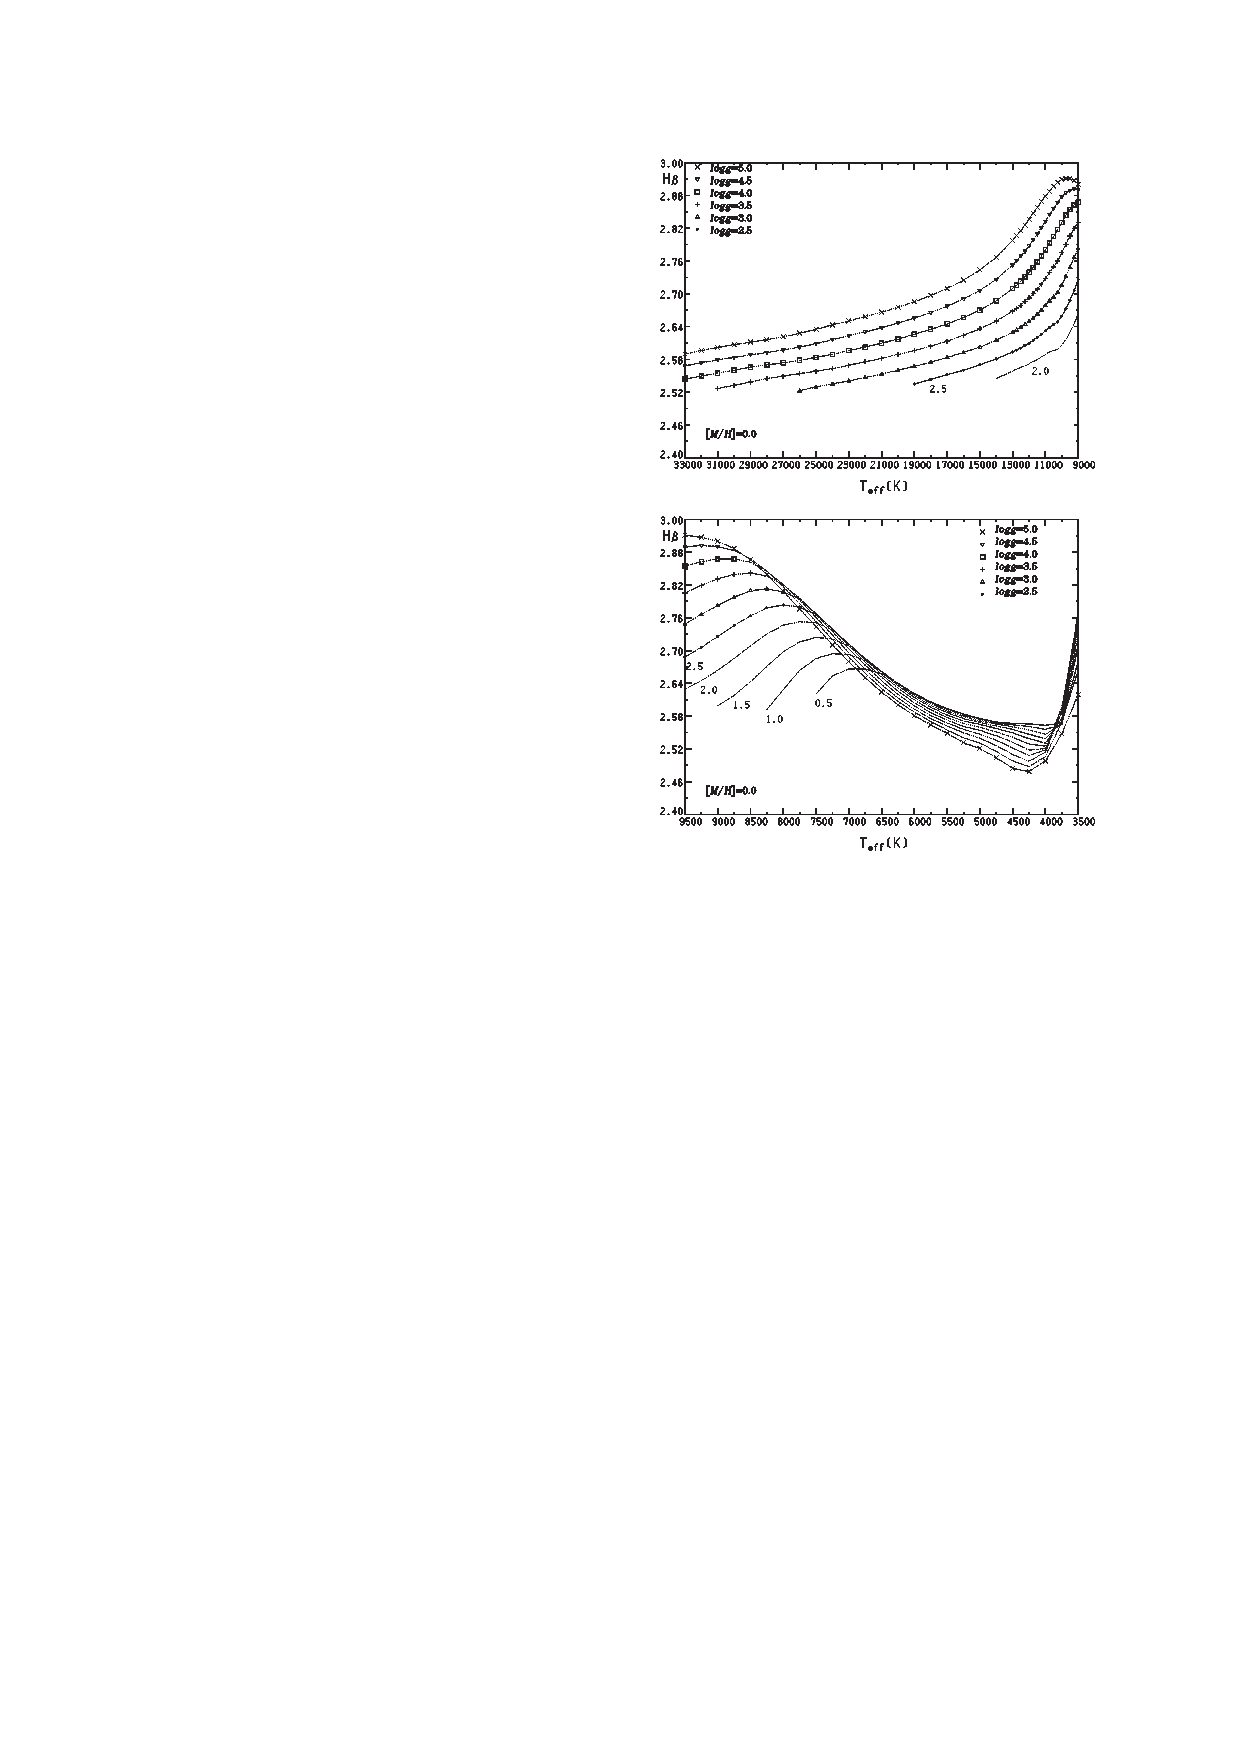
\includegraphics{figures/atlas-beta-index.pdf}
\caption{The Crawford {\Hbeta} index for solar-metallicity stars as predicted from ATLAS9 LTE model by \cite{Castelli-2006}. For BA stars, with $\Teff$ from 7500 to 20,000~K, the {\Hbeta} index is an excellent indicator of surface gravity.}
\label{figure-atlas-beta-index}
\end{figure}

The density increases with surface gravity at a given effective temperature. As the density increases, pressure broadening becomes more important and the observed widths of strong lines such as {\Hbeta} increase. This is shown in Figure~\ref{figure-atlas-hbeta}. Thus, supergiants have narrower lines than giants, and giants have narrower lines than dwarfs.

\begin{table}
\caption{Strömgren-Crawford Diagnostics in BAFG Stars}
\label{table:uvby-beta-diagnostics}
\begin{center}
\begin{tabular}{lcc}
\hline
Parameter&BA&FG\\
\hline
$\Teff$&$b-y$ or $c_1$&$b-y$\\
$\log g$&{\Hbeta}&$c_1$\\
$Z$&&$m_1$\\
\hline
\end{tabular}
\end{center}
\end{table}


The line profile can be measured spectroscopically, of course, but \cite{Crawford-1958} developed a more efficient means to measure its apparent width using filters. He defined two filters centered roughly on the strong {\Hbeta} line, one narrow filter $\beta_n$ with a FWHM of about 3~nm, and one wider filter $\beta_w$ with a FWHM of about 15~nm. Their profiles are shown in Figure~\ref{figure-crawford}. The narrow filter essentially measures the depth of the line in the core and the wider filter essentially measures the surrounding continuum. The ratio of the two, in the form of the {\Hbeta} index, gives an estimate of the relative depth of the line. Figure~\ref{figure-atlas-beta-index} gives a theoretical calibration.

Crawford photometry is used to complement Strömgren photometry.  We have seen that Strömgren photometry of FG stars can be used to measure $\Teff$ (from the $b-y$ color) and $\log g$ (from the $c_1$ index). Strömgren-Crawford photometry for BA stars can be used to measure $\Teff$ (from $b-y$ color and $c_1$ index) and $\log g$ (from the {\Hbeta} index). These diagnostics are summarized in Table~\ref{table:uvby-beta-diagnostics}.

\newslide

\section{Equivalent Width}

\begin{figure}
\footnotesize
\begin{tikzpicture}
\begin{axis}[
   xlabel={$\Delta\nu$ [arbitrary units]},
   ylabel={$R \equiv F_\nu/F_\nu^C$},
   ymin=0.0,
   ymax=1.1,
   minor y tick num=3,
   xmin=-5, 
   xmax=+5,
   minor x tick num=1,
]
\addplot[black,dotted] table[x index=0,y index=2]{figures/line-profile-saturation.dat};
\addplot[black,solid,pattern=north east lines] table[x index=0,y index=4]{figures/line-profile-saturation.dat};
\addplot[black,pattern=north west lines] table {
4.3581814525790505 0
4.3581814525790505 1
3.5 1
3.5 0
};
\end{axis}
\end{tikzpicture}
\caption{An example of the equivalent width. The area between normalized residual flux $R \equiv F_\nu/F_\nu^C$ (solid line) and the normalized continuum (dotted line) is about 0.86 in these arbitrary frequency units. Thus, the equivalent width of the line is 0.86. This is also the area of the rectangle, which has a width of 0.86.}
\label{figure:equivalent-width}
\end{figure}

We can define a hypothetical ``continuum flux'' $F_\nu^c$
at the frequency of a line as the flux we would observe if
the line had no opacity but otherwise the atmosphere was
unchanged. (This is not self consistent; removing a line
will change the temperature structure of an atmosphere.)
Often we will approximate this by simply interpolating the
flux from the continuum on either side of the line.

We can then define the normalized absorption depth $A$ by
\begin{align}
A \equiv 1 - (F_\nu / F_\nu^c),
\end{align}
and also the normalized residual flux $R$ by
\begin{align}
R \equiv (F_\nu / F_\nu^c) = 1 - A.
\end{align}
These are obviously just the fraction of the continuum flux
removed by the line and remaining. In the Sun, we can define
these in terms of the specific intensity as functions of
$\mu$.

As we observe a the spectrum of a star at higher resolution,
each pixel in our detector detectos fewer photons (if the
spectrograph efficiency remains constant), and so the
spectrum becomes noisier. Thus, we often cannot observe at a
sufficiently high resolution to determine the profile of a
line, but instead must measure the equivalent width $W$
defined by
\begin{align}
W = \int_0^\infty A\,d\nu,
\end{align}
or, much more commonly,
\begin{align}
W = \int_0^\infty A\,d\lambda.
\end{align}
The equivalent width is an
integrated quantity, and corresponds to the width in frequency or wavelength of an
imaginary rectangular line that is completely opaque and has the same
``area'' as the real line. This shown in Figure~\ref{figure:equivalent-width}.

One of the most useful properties of the equivalent width is
that it is independent of the spectrograph resolution. This
is because the finite resolution of a spectrograph
effectively acts to convolve the spectrum with a response
function. A little consideration shows that this convolution
broadens the line, but keeps its total area relative to the
continuum constant. However, this constant quantity is
exactly the equivalent width.

%\comment{Figure for EW. Contrast with local broadening
%mechanisms. This section might be better after the local
%mechanisms, and possibly even after the section on LTE
%atmospheres. It might include a derivation of $A$ from
%$a(\mu)$. Gray has some nice comments on the how the optical
%depth effects the treatment of broadening.}

\newslide

\section{The Curve of Growth}

The curve of growth is a plot of the equivalent width
$W$ of an absorption line against the product of the
column density in an absorber $N$ and the oscillator
strength $f$. The product $Nf$ is a measure of how strong a
line is, and ploting this product allows different lines to
be plotted on the same graph by normalizing all of the lines
by this notional strength.

The curve of growth is an important tool for understanding
the behaviour of spectral lines. Historically, it was very
important in abundance measurements, both in stellar
atmospheres and ther ISM, but now it has been largely
replaced by more direct modelling of stellar atmospheres and
ISM absorption profiles.

\begin{figure}
\begin{center}
\begin{tikzpicture}
\begin{scope}
\draw[draw=none,thin,pattern=north west lines](0,0) -- (0,2) -- (4,2) -- (4,0) -- cycle;
\draw[draw=none,thin,pattern=north east lines](0,2) -- (0,3) -- (4,3) -- (4,2) -- cycle;
\draw[thick](0,2) -- (4,2);
\draw[thick](0,3) -- (4,3);
\draw[->]  (2,2) -- (2,4) node[above] {$F_{\nu}$};
%\draw[->] (0,1) -- (2,1) node[above] {$S_\nu$} -- (4,1);
%\draw[->] (4,1) -- (4.5,1) node[above] {$I_{\nu}(T)$} -- (5,1);
\draw (0,1) node[left]{emitting layer};
\draw (0,2.5) node[left]{absorbing layer};
\draw[<->] (4.5,2) -- (4.5,2.5) node[right] {$Z$} -- (4.5,3);
\end{scope}
\end{tikzpicture}
\end{center}
\caption{The geometry of the simple model for the curve of growth. An absorbing layer of thickness $Z$ and density $n$ lies above an emitting layer. We consider only upward rays.}
\label{figure:curve-of-growth-geometry}
\end{figure}

Let's consider a simple model of a uniform line absorbing
layer overlying a continuum emitting layer, as shown in Figure~\ref{figure:curve-of-growth-geometry}.
This is not a
realistic model of an atmosphere -- an atmosphere is not
uniform and the emitting and absorbing layers are intermixed
-- but it is a useful first approximation. Furthermore, we
will assume that the emitted continuum intensity $F_\nu^C$ is sharply peaked
in the outward direction (which allows us to ignore an
integration over solid angle). This allows us to write the
emergent flux as
\begin{align}
F_\nu = F_\nu^Ce^{-\tau},
\end{align}
where $\tau$ is the normal optical depth though the line
absorbing layer. 
The equivalent width is given by
\begin{align}
W 
&= \int_0^\infty\!\!\!d\nu A_\nu\\
&= \int_0^\infty\!\!\!d\nu \left(1 - \frac{F_\nu}{F_\nu^C}\right)\\
&= \int_0^\infty\!\!\!d\nu \left(1 - e^{-\tau}\right).
\end{align}
The optical depth is given by
\begin{align}
\tau(\nu) &= \int\!\! dz\, \alpha(\nu)\\
&=\alpha(\nu) Z\\
&= \left(\frac{\pi e^2}{m_e c}\right) nZ f \phi(\nu)\\
&= \left(\frac{\pi e^2}{m_e c}\right) Nf \phi(\nu)\\
&= T \phi(\nu)
\end{align}
in which the column density $N$ is given by
\begin{align}
N \equiv nZ
\end{align}
and the optical depth integrated over the line $T$ is given by
\begin{align}
T &\equiv \int\!\!d\nu\,\tau(\nu)\\
&=\left(\frac{\pi e^2}{m_e c}\right) Nf.
\end{align}
Thus, we see that in general the equivalent width depends
both on the line strength ($Nf$ or $T$) and on the line profile
($\phi$).

\begin{figure}
\footnotesize
\begin{tikzpicture}
\begin{axis}[
   xlabel={$\Delta\nu$ [arbitrary units]},
   ylabel={$R \equiv F_\nu/F_\nu^C$},
   ymin=0.0,
   ymax=1.1,
   minor y tick num=3,
   xmin=-30, 
   xmax=+30,
   minor x tick num=1,
]
\addplot[black,dashed] table[x index=0,y index=1]{figures/line-profile-saturation.dat};
\addplot[black,dotted] table[x index=0,y index=2]{figures/line-profile-saturation.dat};
\addplot[black,solid] table[x index=0,y index=3]{figures/line-profile-saturation.dat};
\addplot[black,solid] table[x index=0,y index=4]{figures/line-profile-saturation.dat};
\addplot[black,solid] table[x index=0,y index=5]{figures/line-profile-saturation.dat};
\addplot[black,solid] table[x index=0,y index=6]{figures/line-profile-saturation.dat};
\addplot[black,solid] table[x index=0,y index=7]{figures/line-profile-saturation.dat};
\addplot[black,solid] table[x index=0,y index=8]{figures/line-profile-saturation.dat};
\addplot[black,solid] table[x index=0,y index=9]{figures/line-profile-saturation.dat};
\addplot[black,solid] table[x index=0,y index=10]{figures/line-profile-saturation.dat};
\addplot[black,solid] table[x index=0,y index=11]{figures/line-profile-saturation.dat};
\end{axis}
\end{tikzpicture}
\caption{The observed residual flux $R \equiv F_\nu/F_\nu^C$ for the simple model for the curve of growth. The dashed line is the assumed line profile. The dotted line is the continuum. The solid lines are the emergent fluxes $F_\nu$ for total line opacity $T = \int\!\!d\nu\,\tau$ of 1/4, 1, 4, 16, \ldots, 16384.}
\label{figure:profile-saturation}
\end{figure}

We now consider three cases, of increasing line strength.

\begin{enumerate}

\newslide

\item[(a)] Weak lines.

For weak lines, $\tau \ll 1$ and so we can approximate
$e^{-\tau}$ as $1 - \tau$. In this case, we
have
\begin{align}
W 
&= \int\!\!\!d\nu \tau(\nu)\\
&= T \int_0^\infty\!\!\!d\nu' \phi(\nu')\\
&= T
\end{align}
Thus, we have $W = T$, and the curve of growth will be linear.

\newslide

\item[(b)] Lines saturated in the Gaussian core.

Eventually, the line will
\emph{saturate} when the optical depth in the line center is large and the residual flux in this part of the line falls essentially to zero. This can be seen in Figure~\ref{figure:profile-saturation}. In this case, the contribution of the central part of the
line to $W$ will cease to grow and $W$ grows only as
the central part widens. The transition from the optically thick core the the optically thin wings will be abrupt, and the absorption line profile becomes quite rectangular. In Figure~\ref{figure:profile-saturation}, this regime corresponds to $T=16$ to $T=256$

The equivalent width will be
roughly the FW at the point that the optical depth in the
line reaches 1. Thus,
\begin{align}
1 &\approx T \phi(\nu_0 + W / 2)
\end{align}
Since the core is a Doppler profile, we have
\begin{align}
1 &\approx T
\pi^{-1/2}\Delta\nu_0^{-1} \exp(-W^2/4\Delta\nu_0^2)
\end{align}
or
\begin{align}
\exp(W^2/4\Delta\nu_0^2) \approx T \pi^{-1/2}\Delta\nu_0^{-1}
\end{align}
or
\begin{align}
W \propto 2 \Delta\nu_0\left[\ln(T \pi^{-1/2}\Delta\nu_0^{-1})\right]^{1/2}.
\end{align}
This is known as the flat or saturated part of the curve of
growth, as it grows so slowly -- as the square root of the logarithm of the line strength. In Figure~\ref{figure:profile-saturation}, it corresponds to the crowding of lines from about $T=16$ to $T=256$, in which even though the total opacity of the line increases by a factor of 16, the area corresponding to the equivalent width only grows moderately.

\newslide

\item[(c)] Lines saturated in the Lorentzian wings.

Eventually, though, the Lorentzian damping wings become important. Again, approximating the line as a rectangle (although this is now no longer such a good approximation), we have 
\begin{align}
1 \approx T
\frac{\Gamma / 4\pi^2}{(W/2)^2 +
(\Gamma/4\pi)^2},
\end{align}
but when $W \gg \Gamma$, 
\begin{align}
1 \approx T \frac{\Gamma / 4\pi^2}{(W/2)^2},
\end{align}
or
\begin{align}
W \approx \pi^{-1}\sqrt{T\Gamma}
\end{align}
This is known as the square-root or damped part of the
curve. Growth resumes as $\sqrt{T}$, which is faster than in the flat part but not as fast as in the linear part.  In Figure~\ref{figure:profile-saturation}, it corresponds to the crowding of lines above $T=256$, in which the area starts to grow again more rapidly than in the saturated regime.

\end{enumerate}

\newslide

Figure~\ref{figure:curve-of-growth} shows the theoretical curve of growth for the profile in Figure~\ref{figure:profile-saturation}. The linear part is below $\log T \approx 0.5$, the flat part from $\log T \approx 1$ to $\log T \approx 2$, and the square-root part is above $\log T \approx 3$.

\begin{figure}
\footnotesize
\begin{tikzpicture}
\begin{axis}[
   xlabel={$\log T$},
   ylabel={$\log W$},
   ymin=-1,
   ymax=2,
   xmin=-1, 
   xmax=5,
]
\addplot[black,solid] table[x index=0,y index=1]{figures/line-profile-curve-of-growth.dat}
  coordinate [pos=0.25] (A)
  coordinate [pos=0.5] (B)
  coordinate [pos=0.75] (C)
;
\draw (A) node [anchor=south east] {$(a)$};
\draw (B) node [anchor=south ] {$(b)$};
\draw (C) node [anchor=south east] {$(c)$};
\end{axis}
\end{tikzpicture}
\caption{The curve of growth for the profile in Figure~\ref{figure:profile-saturation}. The linear, flat, and square-root regimes are marked by (a), (b), and (c).}
\label{figure:curve-of-growth}
\end{figure}

The form of the curve of growth is important in the practice of determining abundances from absorption lines. Essentially, the idea is that we can measure $W$ and use the curve of growth to determine $T$ with in term gives is the columns density $N$. If we do this for lines of different species, we can measure their relative abundances.

\newslide

\subsection{Propagation of Errors}

However, let us for a moment consider that we will always measure $W$ with some uncertainty $\sigma_W$. How does this translate into errors in $T$ and hence $N$? From propagation of uncertainties, we know
\begin{align}
\sigma_T^2 = \left(\frac{\partial T}{\partial W}\right)^2\sigma_W^2.
\end{align}
Since $W$ is monotonic in $T$, we can simplify this to 
\begin{align}
\sigma_T = \left(\frac{\partial T}{\partial W}\right)\sigma_W.
\end{align}
Next, we can rearrange this equation to give us the relative uncertainties, $\sigma_W/W$ and $\sigma_T/T$, obtaining
\begin{align}
T \left(\frac{\sigma_T}{T}\right) &= W\left(\frac{\partial T}{\partial W}\right)\left(\frac{\sigma_W}{W}\right)\\
\left(\frac{\sigma_T}{T}\right) &= \left(\frac{W \partial T}{T \partial W}\right)\left(\frac{\sigma_W}{W}\right)\\
\left(\frac{\sigma_T}{T}\right) &= \left(\frac{\partial \ln T}{\partial \ln W}\right)\left(\frac{\sigma_W}{W}\right)
\end{align}
Thus, for a given fixed uncertainty in the measurement $\sigma_W/W$, the uncertainty in the total optical depth and the abundance is larger by a factor of the logarithmic derivative $\partial \ln T/\partial \ln W$. This is the inverse gradient in the curve of growth. In the linear regime this factor is 1; in the flat regime this factor is very much greater than 1; and in the square-root regime this factor is 2. Thus, to obtain the smallest relative errors in the abundance, we should favor first lines in the linear regime, then lines in the square-root regime, and probably not even both with lines in the flat regime.

\begin{figure}
\footnotesize
\begin{tikzpicture}
\draw[->] (0,0) -- (0,2) node [left] {$\log W$} -- (0,4);
\draw[->] (0,0) -- (3,0) node [below] {$\log T$} -- (6,0);
\draw(0.5,0.5) -- (1.6,1.6) -- (3.6,2.0) -- (5.6,3.0);

\draw[dashed] (0,1.1) -- (1.1,1.1);
\draw[dashed] (0,0.9) -- (0.9,0.9);
\draw[dotted] (1.1,0) -- (1.1,1.1);
\draw[dotted] (0.9,0) -- (0.9,0.9);

\draw[dashed] (0,1.9) -- (3.1,1.9);
\draw[dashed] (0,1.7) -- (2.1,1.7);
\draw[dotted] (3.1,0) -- (3.1,1.9);
\draw[dotted] (2.1,0) -- (2.1,1.7);

\draw[dashed] (0,2.6) -- (4.8,2.6);
\draw[dashed] (0,2.4) -- (4.4,2.4);
\draw[dotted] (4.8,0) -- (4.8,2.6);
\draw[dotted] (4.4,0) -- (4.4,2.4);

\end{tikzpicture}
\caption{Propagation of errors in a schematic curve of growth. For a given relative error in $W$ (represented by the pairs of dashed lines), the relative error in $T$ (represented by the pairs of dotted lines) is smallest in the linear regime, and then next smallest in the square-root regime, and largest by far in the flat regime.}
\label{figure:curve-of-growth-error}
\end{figure}

This result can be seen graphically. Consider Figure~\ref{figure:curve-of-growth-error}, which shows a segment of a hypothetical curve of growth. We represent three measurements of $W$ each with the same relative error as three pairs of dashed lines. These pairs of lines have the same separations, since the axes are logarithmic. We then obtain the corresponding measurements of $T$ by extending dashed lines from the $\log W$ axis to the curve of growth and then extending dotted lines down to the $\log T$ axis. We see that the relative error in $T$ is smallest in the linear regime, then twice as large in the square-root regime, and much larger in the flat regime.

While the curve of growth was used in early studies of abundances, modern studies fit model fluxes from model stellar atmospheres to observed fluxes, iterating and adjusting the abundances in the atmosphere until the best match is found. Nevertheless, the curve of growth tells us while lines will be most sensitive for determining the abundances: weak unsaturated lines and strong damped lines.

%What are the effects of $\Delta\nu_D$ and $\Gamma$? A large
%$\Delta\nu_D$ makes the line broader by a factor
%proportional to $\Delta\nu_D$, and hence shallower by a
%factor inversely proportional to $\Delta\nu_D$ at a given
%$Nf$. This will delay the onset of saturation in the core.
%Hence, the extent of the linear part of the curve is
%proportional to $\Delta\nu_D$.
%
%The transition from the flat to the square root part of the
%curve occurs when the damping profile becomes more important.
%If a damping profile has a larger value of $\Gamma$, it will
%be wider and will become important sooner. Thus, the
%critical parameter that determines the transition from the
%flat to the square root part is $\Gamma/\Delta\nu_D$; when
%this is higher, the transition occurs sooner.

%%%%%%%%%%%%%%%%%%%%%%%%%%%%%%%%%%%%%%%%%%%%%%%%%%%%%%%%%%%%
%%%%%%%%%%%%%%%%%%%%%%%%%%%%%%%%%%%%%%%%%%%%%%%%%%%%%%%%%%%%

